\lhead{\emph{Capitolo 3}}
\chapter{Case Study: L'approccio ibrido con tecnologie web}

L'approccio ibrido con tecnologie web è stato scelto durante lo svolgimento del tirocinio presso la ditta BigThink SRL, in quanto si adattava meglio ad una serie di tecnologie già utilizzate dall'azienda.
Durante la permanenza in azienda ho svolto il lavoro di Frontend Developer di Web Applications, in particolare mi occupavo dello sviluppo della logica di business di una applicazione e della sua interfaccia.
Una delle politiche dell'azienda era quella di separare la gestione dei dati e la loro memorizzazione lato Backend in modo tale che la parte Frontend sviluppata con il framework Javascript AngularJS si interfacciasse con i dati servendosi solo di API REST.
Data il numero consistente di Web Application sviluppate e il mercato di applicazioni Mobile sempre in crescita, sono stato incaricato dall'azienda di ricercare dei metodi e delle tecnologie che consentissero di portare il lavoro già fatto per le Web Application su dispositivo mobili, in modo tale che l'azienda avesse nuovi servizi da offrire.\\
Tutte le applicazioni sviluppate fino ad allora erano già Responsive Web Application, in azienda si volevano aggiungere funzionalità caratteristiche dei dispositivi mobili tramite l'utilizzo di tecnologie web.\\

Un primo punto di riferimento come tecnologia Web è stato AgnularJS, framework già utilizzato dall'azienda, se fosse stato scelto un altro framework si sarebbe dovuto riscrivere tutto il codice delle Web Application già sviluppate fino a quel punto. A questo punto  si trattava di scegliere le corrette tecnologie per includere al meglio il lavoro già svolto, in particolare un Wrapper che avrebbe consentito un buon sviluppo dell'applicazione partendo da tecnologie web, senza influire su eventuali spese aziendali. 

Per quanto riguarda gli strumenti di sviluppo utilizzati la scelta rimane allo sviluppatore, nel mio caso ho preferito elencarne alcuni secondo me importanti utilizzati all'interno dell'azienda e scoperti durante l'attività di ricerca.

\section{Le Tecnologie Web utilizzate}
Il riferimento per la scelta di tecnologie web è stato il framework AngularJS, il quale è utilizzato a sua volta all'interno di altri framework, come ad esempio Ionic che fornisce degli strumenti per la creazione di interfacce utente. Come Wrapper ho scelto Cordova, in quanto oltre ad essere un progetto open-source fornisce delle API per le funzionalità del dispositivo in linguaggio Javascript. Inoltre esiste un'ultima libreria che richiama le funzionalità di Cordova utilizzando il framwork AngularJS, il che viene molto comodo per il set di tecnologie scelto.

Il framework Ionic per la creazione dell'interfaccia utente è composto oltre da AngularJS da altre tecnologie come un \emph{CSS Preprocessor} che verrà spiegato prima di introdurre nel dettaglio le tencnologie introdotte precedentemente.

\subsection{CSS Preprocessor}

Nei Web Framework che forniscono strumenti per la definizione di interfacce utente un componente che si trova molto spesso e il \emph{CSS Preporcessor} ovvero un preprocessore di fogli di stile.

\emph{In informatica, un preprocessore o precompilatore è un programma (o una porzione di programma) che effettua sostituzioni testuali sul codice sorgente di un programma, ovvero la precompilazione. I più comuni tipi di sostituzioni sono l'espansione di macro, l'inclusione di altri file, e la compilazione condizionale (vedi conditional compilation in inglese). Tipicamente, il preprocessore viene lanciato nel processo di compilazione di un software, e il file risultante verrà preso in input da un compilatore.}
\hspace*{\fill}\cite{wiki:preprocessor} 

\begin{figure}[htbp]
  \centering
    
\includegraphics[scale=0.25]{Figures/sass-logo.png} 
    
\includegraphics[scale=0.75]{Figures/less-logo.png} 
    \rule{35em}{0.5pt}
  \caption[Css Preprocessors]{\textbf{S}intatically \textbf{A}wesome \textbf{S}tyle\textbf{S}heet e \textbf{LESS}}
  \label{fig:CSS Preprocessors}
\end{figure}



Essendo CSS un linguaggio fortemente dichiarativo basato sui markup HTML, fa si che i fogli di stile per interfacce utente diventino molto lunghi e verbosi data la complessità. E di conseguenza la personalizzazione da parte dello sviluppatore che andrà a utilizzare il framework diventa molto difficile.
I CSS preprocessor mettono a disposizione un set di operazioni chiamate MACRO che durante la compilazione verranno sostituite con il linguaggio CSS prorpio. Queste MACRO consentono ad esempio di fare utilizzo di variabili, funzioni, tag parametrici, ereditarietà dei tag, pattern matching, namespaces.

Queste sono solo alcune delle opzioni messe a disposizione dei CSS preprocessors dipende dalle sviluppatore scegliere quello secondo lui più adatto in quanto sul mercato ne esistono diversi, i più famosi e utilizzati sono \textbf{SASS}(\textbf{S}intatically \textbf{A}wesome \textbf{S}tyle\textbf{S}heet) e \textbf{LESS}(write \textbf{LESS} do more) \ref{fig:CSS Preprocessors}.

\subsection{AngularJS}

\begin{wrapfigure}{r}{0.40\textwidth}
  \vspace{-65pt}
  \begin{center}
    
\includegraphics[scale=0.40]{Figures/angular-logo.png}
  \end{center}
  \vspace{-10pt}
  \caption{\\AngularJS framework logo}
  \label{fig:AngularJS}
  \vspace{10pt}
\end{wrapfigure}

\paragraph*{Definizione}
AngularJS è un framework Javascript che segue il pattern MVC(\ref{sec:MVC}) ideato da \emph{Minsko Hevery}(Google) che estende il linguaggio HTML in un formato più espressivo e leggibile. Consente di aggiungere nuovi tag HTML speciali in modo da sincronizzare la parte scritta in Javascript senza manualmente aggiornare la view, in modo tale da rendere indipendente la logica della applicazione. Angular semplifica la scrittura di codice Javascript rendendo il codice dell'applicazione più efficiente e leggibile.
\paragraph*{Caratteristiche e Componenti}
AngularJS interpreta il design pattern MVC grazie al quale si arricchisce con una serie di caratteristiche molto interessanti:
\begin{description}

\item[Data Binding] Il Data Binding in AngularJS è la sincronizzazione automatica dei dati tra modello e vista. In modo in cui AngularJS implementa il data bindign consente di trattare il modello come SSOT(\cite{wiki:SSOT}). La vista è la proiezione del modello in ogni momento, quando il modello cambia la vista riflette il cambiamento e viceversa. 
La maggior parte dei sistemi di templating sincronizzano i dati in una sola direzione: si fondono componenti del template e modello insieme in una vista. Quando si verifica la fusione, le modifiche al modello o sezioni correlate della vista vengono NON si riflettono automaticamente nella vista. Peggio ancora, le eventuali modifiche che l'utente fa nella vista non si riflettono nel modello. Ciò significa che lo sviluppatore deve scrivere del codice apposito che sincronizza costantemente la vista con il modello e il modello con la vista.

\begin{figure}[htbp]
  \centering
    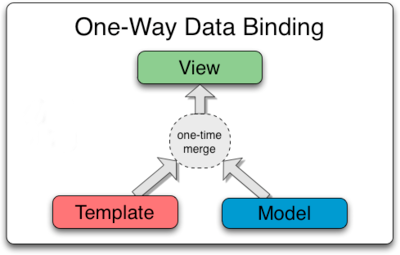
\includegraphics[scale=0.5]{Figures/one-way-data-binding.png} 
    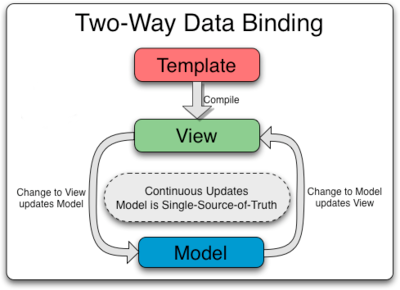
\includegraphics[scale=0.5]{Figures/two-way-data-binding.png} 
    \rule{35em}{0.5pt}
  \caption[Data Bindings]{Come è strutturato un classico data binding, e come invece è fatto in AngularJS}
  \label{fig:Data Binding}
\end{figure}

In particolare come si vede nell'esempio \ref{lst:directives-example} il binding dalla vista al modello è effettuato tramite la direttiva \emph{ng-model = "nome-del-modello"}, mentre dal modello alla vista si utilizza la sintassi \emph{ \{\{nome-del-modello\}\} }.

Il systema dei templates di AngularJS funziona in modo differente. In primo luogo il modello (che è l'HTML non compilato insieme a  markup o direttive supplementari) viene compilato sul browser. Il passo di compilazione produce una live view(vista). Eventuali modifiche alla vista si riflettono immediatamente nel modello, e le eventuali modifiche nel modello vengono propagate alla vista. Il modello è il SSOT per lo stato dell'applicazione, semplificando notevolmente il modello di programmazione per lo sviluppatore. Si può pensare di vista semplicemente come una proiezione istantanea del modello.

Poiché la vista è solo una proiezione del modello, il controller è completamente separato dal punto di vista e completamente allo scuro di essa. Questo rende i test dell'applicazione molto semplici, in quanto è facile testare il controller indipendentemente dalla vista e dalla relativa dipendenza dal DOM / browser web.

\item[Scope] Lo \emph{Scope} è un oggetto che si riferisce al modello dell'applicazione. E' il contesto dove vengono eseguite le espressioni. Esistono più scope all'interno dell'applicazione e sono organizzati in maniera gerarchica ad imitare la struttura del DOM dell'applicazione. Infine sullo scope si può osservare una espressione e propagare eventi.
I vari scope di una applicazione in AngularJS sono i nodi centrali a cui ruota attorno tutta la logica dell'applicazione, grazie a loro e possibile la comunicazione tra vista e modello con l'utilizzo del data binding. Per una trattazione più approfondita si rimanda alla documentazione di AngularJS(angularjs.org).

\item[Controller] i controller in AngularJS hanno il compito di gestire la logica di una determinata sezione dell'applicazione. Quando un controller viene dichiarato su una parte del DOM tramite la direttiva \emph{ng-controller} come nell'esempio \ref{lst:newController} AngularJS crea un nuovo oggetto Javascript associandogli un nuovo scope che potrà essere inserito all'interno del controller tramite la dependency injection. 

\begin{lstlisting}[caption={Associazione tra un elemento del DOM e un controller}, label={lst:newController}]
	<div id="header" ng-controller = "HeaderController"></div>
\end{lstlisting}
In generale ci sono alcune regole da seguire per la creazione dei controller, le quali non sono obbligatorie ma sono considerate come si dice in gergo \emph{Best Practices}:
I controller devono essere usati per:
\begin{itemize}
\item Configurare lo stato iniziale dello scope.
\item Aggiungere comportamento allo scope(funzioni, modelli, oggetti)
\end{itemize}
Mentre i controller non devono essere usati per:
\begin{itemize}
\item Manipolare elementi del DOM
\item Formattare input e output
\item Condividere codice tra i vari controller.
\item Gestire il ciclo di vita degli altri componenti(creazione di nuove istanze)
\end{itemize}

\item[Dependency Injection] per una trattazione generale dell'argomento rimandiamo all'appendice \ref{app:DepInj}. AngularJS ha già al suo interno un meccanismo che gestisce la Dependency Injection. Il principale scopo per cui AngularJS è stato dotato di questa caratteristica è per avere la possibilità di suddividere in moduli separati l'applicazione dove ognuno di essi può essere iniettato all'interno degli altri e vice versa. Un esempio moto semplice di Dependency Injection in AngularJS è all'atto della creazione dell'applicazione. Nell'esempio \ref{lst:appCreation} il metodo \textit{angular.module()} prende due argomenti: il primo è il nome del modulo che si vuole creare, mentre il secondo è un array con tutti i moduli di cui è composto la nostra applicazione. Viene creato quindi un riferimento ai moduli inclusi e non un istanza diretta.  
\begin{lstlisting}[caption = {Creazione di una applicazione in AngularJS con le relative dipendenze}, 
				   label = {lst:appCreation}]
	var testApp = angular.module("testApp",['ngRoute','customModule']);
\end{lstlisting}

Oltre ai moduli AngularJS da la possibilità di usare la propietà della Dependency Injection sui tipi base forniti dal linguaggio, ovvero:
\begin{itemize}
\item Value
\item Factory
\item Service
\item Provider
\item Constant
\end{itemize}
Un esempio di Dependency Injection di questi tipi avviene molto frequentemente nelle applicazioni all'interno dei controller (\ref{lst:controllerExample})

\begin{lstlisting}[caption = {Un esempio di creazione di un modulo e la sua inclusione all'interno di un altro}, 
				   label = {lst:controllerExample}]

angular.module("CustomModule",[])
.service("CustomService",function(){
	this.customMethod = function(value){
		return value + " from customMethod in CustomService";	
	}
});

angular.module("testApp",[
	'CustomModule'
]).controller("HomeController", function(CustomService){
	CustomService.customMethod("Marco");
});


\end{lstlisting}

\item[Service] si è visto come il meccanismo di Dependency Injection possa rendere disponibile all'interno dell'applicazione tutti i componenti forniti da un specifico modulo. Fatta eccezione per i \emph{service} ogni volta che si richiama un componente tramite Dependency Injection dal riferimento viene creata una nuova istanza della classe. I service invece sfruttano quello che è chiamato in Javascript il \emph{Singleton Object}, ovvero, l'istanza di un oggetto di tipo service avviene soltanto una volta, e il riferimento all'interno dell'applicazione è univoco verso lo stesso oggetto(figura \ref{fig:AngularJS-Singleton}). Inoltre soltanto quando il service dipende dall'applicazione viene creata l'istanza dell'oggetto(\emph{Lazy Initialization}).

\begin{figure}[htbp]
  \centering
    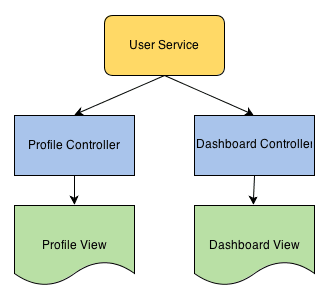
\includegraphics[scale=0.75]{Figures/angularjs-service-singleton-diagram.png}  
    \rule{35em}{0.5pt}
  \caption[AngularJS Singleton]{Schema di come è strutturato un service all'interno di AngularJS}
  \label{fig:AngularJS-Singleton}
\end{figure}

I service possono essere creati dallo sviluppatore oppure AngularJS ne mette a disposizione già alcuni, come ad esempio \emph{\$http} che è uno dei più usati per lo scambio dei dati attraverso l'omonimo protocollo. Altro uso dei service può essere quello dello scambio dei dati attraverso i controller, genericamente in una applicazione che si interfaccia con dei servizi backend e buona norma associare ad ogni servizio corrispettivo un service di AngularJS.

\item[Provider/Factory/Service] una trattazione separata di queste tre caratteristiche di AngularJS potrebbe risultare difficile da comprendere. Avendo spiegato cosa è un service la trattazione prosegue su altri due componenti strettamente correlati: i Factory e i Provider.
Tra questi tre componenti esiste una specie di gerarchia : i \textit{service} sono degli oggetti singleton creati tramite una \textit{factory}. Le \textit{factory} sono funzioni che a sua volta sono create tramite un \textit{provider}. I \textit{provider} sono dei costruttori che hanno a disposizione un metodo \emph{\$get} il quale contiene la \emph{service factory} che ritorna l'istanza del service.

In questo modo AngularJS si garantisce una forte modularizzazione dei componenti, e la ricerca dei corretti riferimenti da parte della Dependency Injection. Inoltre tramite il provider è possibile configurare, se previsto, i servizi dell'applicazione scrivendo un opportuno codice parametrico.

\item[Directives] una delle caratteristiche più rilevanti di AnagularJS è sicuramente quella di poter creare dei tag HTML personalizzati, oltre a quelli già previsti dal framework. Questi tag speciali sono chiamati directives o direttive. AngularJS si serve delle direttive per poter strutturare l'applicazione sulla vista HTML, ovvero ci sono dei tag speciali previsti dal framework che definiscono il nome dell'applicazione(\textit{ng-app}), i controller da utilizzare(\textit{ng-controller}), i modelli di riferimento(\textit{ng-model}) e il contenitore dove processare le viste(\textit{ng-view}) come nell'esempio \ref{lst:directives-example}:
\begin{lstlisting}[language=html,caption={Un esempio delle direttive standard di AngularJS},
				   label={lst:directives-example}]
 <html ng-app = "myApp">
   <head></head>
   <body>
     <div ng-controller = "InfoController">
       <input name = "inputFirstName" ng-model = "user.firstName">
       <input name = "inputSecondName" ng-model = "user.secondName">
       <div class = "showInfo">
	     Hello my name is {{user.firstName}} {{user.secondName}}			
       </div>
     </div>
   </body>
 </html>
\end{lstlisting}

Inoltre possiamo definire direttive personalizzate alle quali possiamo associare un relativo comportamento(\ref{lst:custom-directive}). Una cosa che è concessa nelle direttive e non nelle altre strutture di AngularJS è la manipolazione del DOM, solo al loro interno è possibile scrivere codice che interagisca direttamente con gli elementi della vista.
\begin{lstlisting}[language=html,caption={Un esempio di direttiva personalizzata},
				   label={lst:custom-directive}]
 angular.module("myApp")
 .directive("myPersonalTag",funcIonic: Advanced HTML5 Hytion(){
	return{
		link: function(scope, element, attrs){
			//directive main istructions		
		}	
	} 
 });
\end{lstlisting}

Una nota di sintassi particolare per le direttive riguarda il loro nome, come osserviamo il nome delle direttive nell'esempio \ref{lst:directives-example} è separato dal trattino alto(\emph{dash}) mentre nella definizione tramite codice AngularJS è scritta in \emph{camelCase}. Questa è un convenzione che il framework adotta per evitare errori di sintassi all'interno del codice da parte del parser.
Oltre alle caratteristiche principali con le direttive si hanno a disposizione molte più opzioni. Si rimanda l'approfondimento qui : \cite{angularjs:directives} per un trattazione più approfondita.

\end{description} 


\subsection{Ionic}

\begin{wrapfigure}{r}{0.40\textwidth}
  \vspace{-65pt}
  \begin{center}
    
\includegraphics[scale=0.35]{Figures/ionic-logo.png}
  \end{center}
  \vspace{-10pt}
  \caption{Ionic Framework Logo}
  \label{fig:IONIC}
  \vspace{5pt}
\end{wrapfigure}

IONIC fa parte della famiglia degli UI Framework per creazione di interfacce utente per dispositivi mobili e applicazioni ibride e si serve delle tecnologie web AngularJS, Sass e HTML5.
Il lavoro da svolgere per chi vuole utilizzare questo tipo di framework e quello di scegliere i vari componenti messi a disposizione e di comporli per creare l'applicazione finale. Generalmente si parte da un template messo a disposizione dal framework e si compone l'applicazione. La modularità dei componenti di IONIC è data dal sistema di direttive di AngularJS, tutti i componenti sono sviluppati in direttive separate e come si può notare tutti i rispettivi tag HTML iniziano con il prefisso \textit{ion} o \textit{ionic}. 
La caratterizzazione di un framework di questo tipo dipende dal suo stile e design e sta allo sviluppatore(o  grafico) decidere quale in questo caso il più bello per l'applicazione. IONIC inoltre mette a disposizioni diverse caratteristiche che possono influenzare la sua scelta:
\begin{description}
\item[CSS Components]
Sono dei componenti statici creati tramite HTML e CSS come bottoni, barre di navigazione, liste, tabelle che possono essere assemblati tra di loro come i componenti di una pagina web. I CSS di IONIC mettono a disposizione classi che possono cambiarne forma, dimensione e colore che a loro volta possono essere combinate.
Per personalizzazioni più avanzate e possibile seguire una guida messa a disposizione dal framework che spiega come modificare i file di Sass e che caratteristiche si va a cambiare(come ad esempio i colori standard).
\item[Javascript Components]
Al fine di offrire una esperienza di una applicazione mobile all'utente, IONIC offre delle estensioni in ANgularJS che ricalcano quelle che sono le operazioni e le interfacce più comuni sui i dispositivi mobili. Ispirato ai sistemi iOS e Android questo framework mette a disposizione componenti come gestori di eventi, paginazione dei contenuti, popup di sistema, touch gestures, menu laterali, scorrimento di pagine il tutto nello stile di una applicazione mobile vera e prorpia.
\item[Ionicons]
IONIC prevede un set di icone standard che possono essere utilizzate all'interno dei componenti e personalizzate a proprio piacimento.

\end{description} 
\section{Il Wrapper Framework}
Come spiegato nella sezione \ref{sec:appAndFramework} per lo sviluppo di applicazioni ibirde si necessita di un framework che possa in qualche modo tradurre il linguaggio originale in quello della specifica piattaforma.
Nel caso qui studiato si ha bisogno di un framework che possa ospitare tecnologie web e che abbia un interfaccia verso le funzionalità del dispositivo. Si ribadisce che non tutti i framework possono essere usati su tutte le piattaforme, bisogna scegliere con accortezza di quale servirsi.
Data la mia formazione come sviluppatore web presso l'azienda BigThink SRL ho scelto di utilizzare il framework \emph{Cordova} per i seguenti motivi:
\begin{itemize}
\item E' un framework che si adatta a sviluppatori web che vogliono portare le proprie applicazioni su dispositivi mobili, in quanto fornisce le varie API per le funzionalità del dispositivo in linguaggio Javascript.
\item E' open-source quindi costi di licenza nulli per l'azienda e per lo sviluppatore ed inoltre e seguito da una community popolata e attiva.
\item Supporta 16 piattaforme diverse con oltre 20 plugin per interagire con il dispositivo, assieme ad altre librerie per la creazione di plugin personalizzati.
\item Si integra al meglio con AngularJS grazie ad una libreria chiamata \emph{ng-cordova}(\ref{sec:ngCordova}).
\end{itemize}

\subsection{Cordova/Phonegap}

\begin{wrapfigure}{r}{0.40\textwidth}
  \vspace{-65pt}
  \begin{center}
    
\includegraphics[scale=0.35]{Figures/cordova-logo.png}
  \end{center}
  \vspace{-10pt}
  \caption{\\Cordova Framework Logo}
  \label{fig:Cordova}
  \vspace{-30pt}
\end{wrapfigure}


Per chi magari è nuovo nel settore delle applicazioni multi-piattaforma, o per chi ci è entrato da poco 	avrà fatto sicuramente confusione tra queste due nomenclature \texttt{Cordova} e \texttt{Phonegap}, ecco quindi una delucidazione sul fatto.

\subsubsection{Storia}
Phonegap è stato creato nel 2009 da una startup chiamata \emph{Nitobi} come progetto open-source. Si proponeva di fornire un metodo per l'accesso alle funzionalità native del dispositivo tramite il meccanismo di wrapping che è stato discusso nel capitolo precedente a proposito dei framework. L'obiettivo di questa piattaforma era appunto quello di poter creare delle applicazioni che potessero essere usate nei dispositivi mobili, tramite l'utilizzo di tecnologie web come HTML5, CSS e Javascript, ma con ancora la possibilità di accedere alle funzionalità native del dispositivo.\\
Nel 2011 \emph{Adobe} ha acquisito la startup Nitobi assieme ai diritti di Phonegap, e il codice open-source della piattaforma è stato donato all'\emph{Apache Software Foundation} con il nome di \texttt{Cordova}

\subsubsection{Differenze}
La vera differenza tra \texttt{Cordova} e \texttt{Phonegap}, viene descritta da \emph{Adobe} analogamente come la differenza tra \texttt{Blink}\footnote{Blink è la web browser engine di Google Chrome\cite{wiki:blink}} e \emph{Google Chrome}. Ovvero \emph{Cordova} e il cuore della piattaforma mentre \emph{Phonegap} aggiunge a \emph{Cordova} delle funzionalità proprietarie di \emph{Adobe}.\\
Personalmente ho scelto di utilizzare \emph{Cordova} per essere libero da qualsiasi vincolo proprietario.

\subsubsection{Cordova Core}
Cordova quindi offre una serie di potenti API in linguaggio Javascript per poter accedere alle funzionalità native del dispositivo. In difesa dello sviluppo nativo alcuni programmatori accusano \emph{Cordova} di non possedere tutte le possibilità di accesso a basso livello che invece si avrebbero. \emph{Corodova} è una realtà open-source e in quanto tale si è evoluta nel tempo offrendo sempre più funzionalità che hanno chiuso i divario che si credeva esservi tra questi due tipi di approcci.\\
Infine per quanto riguarda lo sviluppo dei plugin verso il futuro, la comunità open-source di \emph{Cordova} sta spronando gli sviluppatori a creare nuove funzionalità sempre più generiche, in modo tale che con l'evolversi delle tecnologie, e soprattutto dei browser web, siano sempre compatibili.

\subsection{ngCordova}
\label{sec:ngCordova}
\begin{wrapfigure}{r}{0.40\textwidth}
  \vspace{-65pt}
  \begin{center}
    
\includegraphics[scale=0.35]{Figures/ngcordova-logo.png}
  \end{center}
  \vspace{-10pt}
  \caption{\\ngCordova Logo}
  \label{fig:ngCordova}
  \vspace{0pt}
\end{wrapfigure}

Il perché in questa tesi si parli di \emph{Cordova} e \emph{AngularJS} è dato dall'esistenza di \texttt{ngCordova}. Questa libreria nasce da una idea di Paolo Bernasconi e Max Lynch che hanno avuto l'idea(geniale) di unire la l'efficenza e la potenza di \emph{AngularJS} con la versatilità di \emph{Cordova}. Ne è nato un framework per lo sviluppo di applicazioni ibride direttamente collegato alle funzionalità del dispositivo gestibile tramite il codice efficiente di \emph{AngularJS}.\\
Per chi vuole sviluppare applicazioni ibride multi piattaforma, questa libreria rende decisamente più rapido ed efficiente il processo di sviluppo.

\section{Strumenti di sviluppo}

\subsection{Il trio Magico}
La mia scelta delle tecnologie da utilizzare per lo sviluppo ibrido di applicazioni multi piattaforma si è incentrata soprattutto sull'efficienza e la compatibilità. Decidendo di utilizzare \texttt{AngularJS} + \texttt{Cordova} + \texttt{ngCordova} ottengo un ambiente di sviluppo rapido ed efficiente, in quanto tutti e tre i framework sono stati sviluppati per una stretta collaborazione, e allo stato dell'arte attuale delle tecnologie penso che sia una delle scelte migliori e rapide di sviluppo.

\subsection{Package Manager}
Bower è un package manager, ci consente di organizzare al meglio le librerie all'interno del nostro progetto. Tramite il file \emph{bower.json} possiamo specificare tutti i dettagli del nostro progetto e dinamicamente aggiornare la lista delle librerie installate. Inoltre se stiamo lavorando con una struttura di cartelle specifica, come ne mio caso, possiamo specificare la posizione di dove verranno scaricate le librerie tramite il file \emph{.bowerrc}. In ambito web non esiste libreria che non possa essere scaricata con bower, sostanzialmente possiamo ottenere qualsiasi cosa presente su \emph{Github}.
-- Codice Bower.json --
-- Codice .bowerrc --

\subsection{Task Runner}

Grunt/Gulp \texttt{Grunt} e \texttt{Gulp} sono due esempi di \emph{task-tunner}. Ho voluto nominarli entrambi nella mia tesi in quanto il primo l'ho usato durante la mia esperienza di tirocinio, il secondo invece è usato dal framework  Ionic per la gestione di tutti i suoi file. Attualmente esistono due schiere di programmatori che sostengono che uno sia meglio dell'altro, personalmente preferisco grunt perché ha un logo più bello(hahaha).\\
Il ruolo dei task-runner non è ben preciso in quanto sono molto versatili e "assemblabili", in quanto per eseguire determinate operazioni necessitano dei loro plugin specifici. Ad esempio se nel mio progetto avessi bisogno di verificare la sintassi di Javascript, concatenare i file di progetto e le librerie, minificarli e spostarli in una cartella differente (ho potuto osservare durante il mio tirocinio che queste operazioni sono molto comode nel tipo di approccio che si ha nello sviluppo di una applicazione ibrida con tecnologie web) devo prima scaricare nel mio progetto ognuno di essi. Questo procedimento può sembrare poco efficiente, in realtà se disponiamo del \emph{Node Package Manager} NPM tutta la lista dei plugin installati nel progetto e registrata su un file \emph{package.json}. Inoltre una funzionalità molto significativa che hanno i task-runner è quella del \texttt{Live Reload}, ovvero sono in grado di vedere se ci sono stati cambiamenti nel nostro progetto e automaticamente eseguire le operazioni stabilite.

\subsection{IDE}
Ho scelto di usare una \emph{Integrated Develop Enviroment}(IDE) per lo sviluppo della mia applicazione in modo tale da tenere sotto controllo tutti i file del mio progetto e per poterli organizzare in una struttura di tipo modulare. Abbiamo constatato che prima di un deploy dell'applicazione ci sono una serie di operazioni che dobbiamo eseguire affinché il nostro progetto sia completo. Per fare questo ci serviamo di strumenti chiamati \emph{Tesk-Runner}.

- Gestione dei progetti -\\
- Organizzazione -\\
- Test -\\
- Deploy -\\
Questi concetti spiegati in modo generale per poi dire nelle varie sezione come sono stati effettivamente applicati.

Tra i diversi IDE disponibili ho scelto di usare \emph{NetBeans} in quanto può predisporre di un ambiente adatto allo sviluppo di applicazioni multi-piattaforma. In particolare è possibile partire da un modello di progetto basato su \emph{Cordova} oppure semplicemente in \emph{HTML5} ed inoltre è molto semplice configurare le SDK dedicate per il deploy sui vari sistemi operativi.

\subsubsection{Creazione}
Tramite NetBeans inizializziamo un nuovo progetto basato si Cordova.
-- Immagine nuovo progetto --\\
-- Immagine scelta del template --
In NetBeans non abbiamo il templateAbbiamo constatato che prima di un deploy dell'applicazione ci sono una serie di operazioni che dobbiamo eseguire affinché il nostro progetto sia completo. Per fare questo ci serviamo di strumenti chiamati \emph{Tesk-Runner}. fornito da Ionic, ma possiamo inizializzare tramite terminale il progetto e poi importarlo nell'IDE. Facendo questa operazione dobbiamo avere l'accortezza di aggiornare le impostazioni del progetto all'interno di NetBeans.
-- Immagine progetto --
Qui abbiamo i risultato del nostro progetto dal quale partire per lo sviluppo.

\subsubsection{Inclusione di Librerie esterne}
Nei progetti per applicazioni multi piattaforma che utilizzano tecnologie web può risultare utile includere delle librerie esterne(spesso in linguaggio Javascript), che con questo tipo di tecnologia, questa operazione risulta molto rapida e intuitiva. \\
Semplicemente come si agisce nei siti web, si inserisce uno script all'interno della pagina \emph{index.html} che va a includere il file della libreria desiderate.

\begin{lstlisting}[language=html]
	<script src = "lib/mylibrary/dist/mylibrary.min.js"></script>
\end{lstlisting}

Con NetBeans possiamo utilizzare in fase di configurazione e anche successivamente uno strumento che automaticamente include librerie da lui elencate, il quale è molto utile ma ovviamente non dispone di tutta la varietà presente in rete. uno strumento molto potente, usato dalla stragrande maggioranza degli sviluppatori web è \texttt{Bower}.

\subsubsection{Deploy}
L'operazione di \emph{Deploy} in italiano "schierare", nel nostro caso prende il significato di produrre una versione della nostra applicazione, che può essere finale oppure no. Nello sviluppo di applicazioni ibride multi piattaforma abbiamo a disposizione 3 opzioni per fare questa operazione.

\begin{description}
\item[Delploy sul Browser] Ovvero andiamo a vedere quella parte di applicazione che non necessita di essere sul dispositivo per poter funzionare. Sostanzialmente visualizziamo solo il livello delle tecnologie web, e lo possiamo correggere e/o visionare come se fosse un normale sito web. In questa modalità però non disponiamo ad esempio dell'interazione con le funzionalità native del dispositivo, si tratta di un modo rapido per avere una vista su quella che sarà l'interfaccia dell'applicazione.

\item[Simulazione] Ogni IDE consente un meccanismo di simulazione di un dispositivo sulla propria macchina. In questa modalità possiamo vedere realmente come sarà la nostra applicazione su un dispositivo, ma in realtà l'hardware di riferimento sarà quello della nostra macchina(il simulatore si occupa di mettere in comunicazione tutte le componenti). E' una modalità che si avvicina molto alla rappresentazione reale della nostra applicazione ma il processo di simulazione per un computer di fascia media comporta una attesa anche di minuti per visionare il risultato, e dato che dovremo ripetere questa operazione diverse volte perché può darsi che si debba correggere il codice(cosa molto frequente), diventa molto dispendioso attendere tutte le volte così tanto tempo.

\item[Installazione su Dispositivo] Quasi tutti i sistemi operativi ad eccezione di iOS, concedono di installare applicazioni direttamente da PC. Nel caso di Android che ho preso in esame, è molto semplice fare un \emph{Deploy} su dispositivo. Tramite \emph{NetBeans} bisogna configurare le SDK e scegliere il proprio dispositivo connesso tramite usb. Nel caso di iOS \emph{Apple} non concede l'installazione di applicazioni da origini sconosciute, a meno che non siano registrate sul Apple Store, pagando una tassa annuale di 99\$.

\end{description}

Quando il nostro progetto prende forma i file all'interno di esso cominciano a diventare consistenti e organizzarli diventa sempre più complesso. E buona norma di programmazione separare il proprio progetto in più file, ma al momento della consegna bisogna anche ricomporli e assemblarli nella maniera corretta. Inoltre se usiamo \emph{Ionic} e abbiamo modificato i fogli di stile dobbiamo ricordarci di ri-compilare i file \emph{SASS}.\\

\subsubsection{Live Debug}
Una volta che l'applicazione è in esecuzione in una delle modalità descritte precedentemente ci si preoccupa di controllare che il codice che si ha scritto funzioni correttamente. Per eseguire un buon \emph{Debug} di questo tipo di applicazione è sufficiente disporre di uno strumento molto semplice \emph{Google Chrome}, infatti tramite questo web browser a diffenza di altri possiamo osservare il comportamento della nostra applicazione sui vari dispositivi(anche in fase di simulazione) come se stessimo facendo una normale ispezione di una pagine web. Ovviamente se l'applicazione è in \emph{Deploy sul Browser} il problema non si pone, qualsiasi browser può andare(anche se personalmente consiglio Google Chrome o Mozilla Firefox).

\section{SDK}
Un \texttt{Software Developement Kit} in generale è un insieme di strumenti per lo sviluppo e la documentazione del software\cite{wiki:sdk}. Questi strumenti vengono rilasciati dalla casa produttrice di una certa piattaforma come librerie di riferimento per lo sviluppo di software specifico di essa. La loro distribuzione avviene in uno specifico linguaggio a seconda della piattaforma ed è sempre affiancata da una documentazione molto accurata. 
Per lo sviluppo di applicazioni ibride avremo bisogno di ciascuna \emph{SDK} per ogni sistema operativo sul quale vorremo la nostra applicazione; ad esempio se volessimo la nostra applicazione per \emph{iOS} e \emph{Android} dovremmo scaricare entrambe le \emph{SDK}(scritte rispettivamente in C++/Swift e Java) indicando dove si trovano all'interno del notro computer. \emph{NetBeans} dispone di una interfaccia molto semplice da usare per impostare i percorsi delle \emph{SDK} ma non di tutte le piattaforme; se volgiamo impostare un'altra piattaforma non indicata nell'IDE dobbiamo seguire le istruzioni fornite da \emph{Cordova}.